\chapter{More on Pipeline}

Here we continue the discussion on pipeline hazards. 

\section{Data Hazards}
Data hazards occur when the pipeline must be stalled because one step must wait for another to complete. To put it simply, this happens because a previous step has not finished data manipulation, while a following step requires the result from the previous step. This leads to data hazards.

Data hazards arise from the dependence of one instruction on an earlier one that is still in the pipeline. There are two main types of data hazards:

The first type is the Read After Write (RAW) data hazard. This occurs when an instruction needs to read a value that has not yet been written by a previous instruction. For example, as shown below, the \verb|add| instruction requires a value that is produced by the preceding \verb|sub| instruction, but \verb|sub| will only write the result to the register during its final pipeline stage.

\begin{center}
  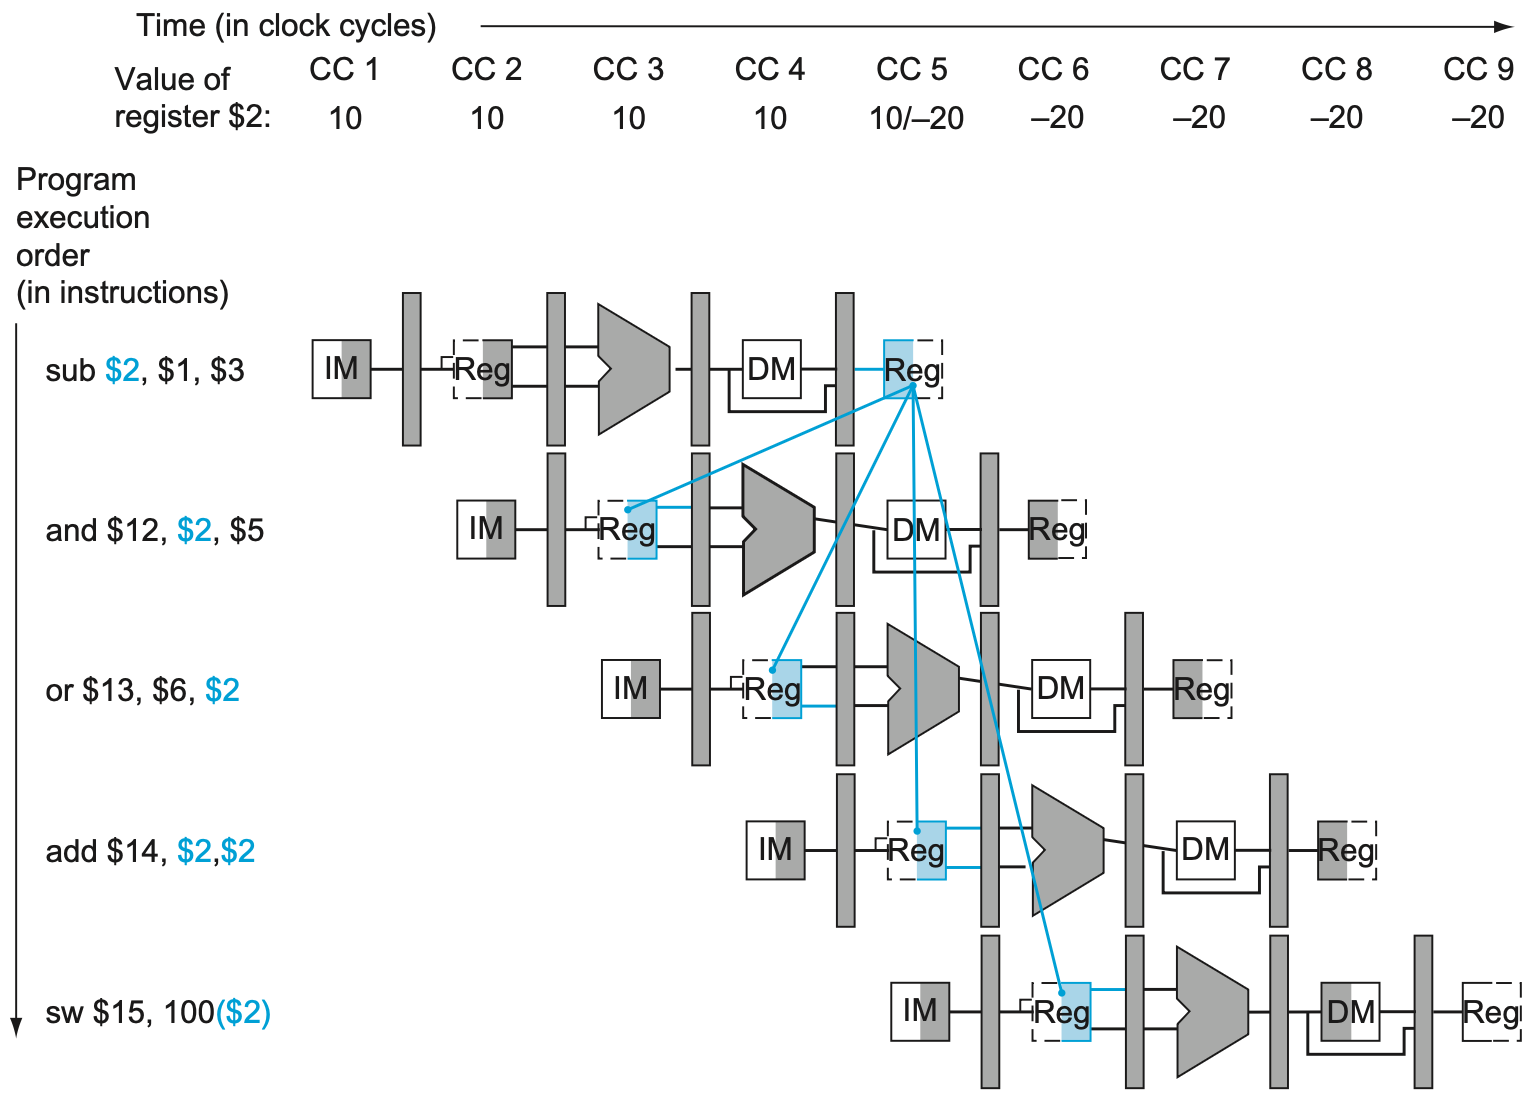
\includegraphics[width=0.8\textwidth]{Figure/pipeline_raw.png}
\end{center}

The second type is the Load-Use data hazard. This occurs when an instruction needs to use data that is being loaded from memory by a previous instruction, but the load (\verb|lw|) operation will only complete at the final pipeline stage. As shown below, the \verb|sub| instruction depends on the result of the \verb|lw| instruction, leading to a data hazard.

\begin{center}
  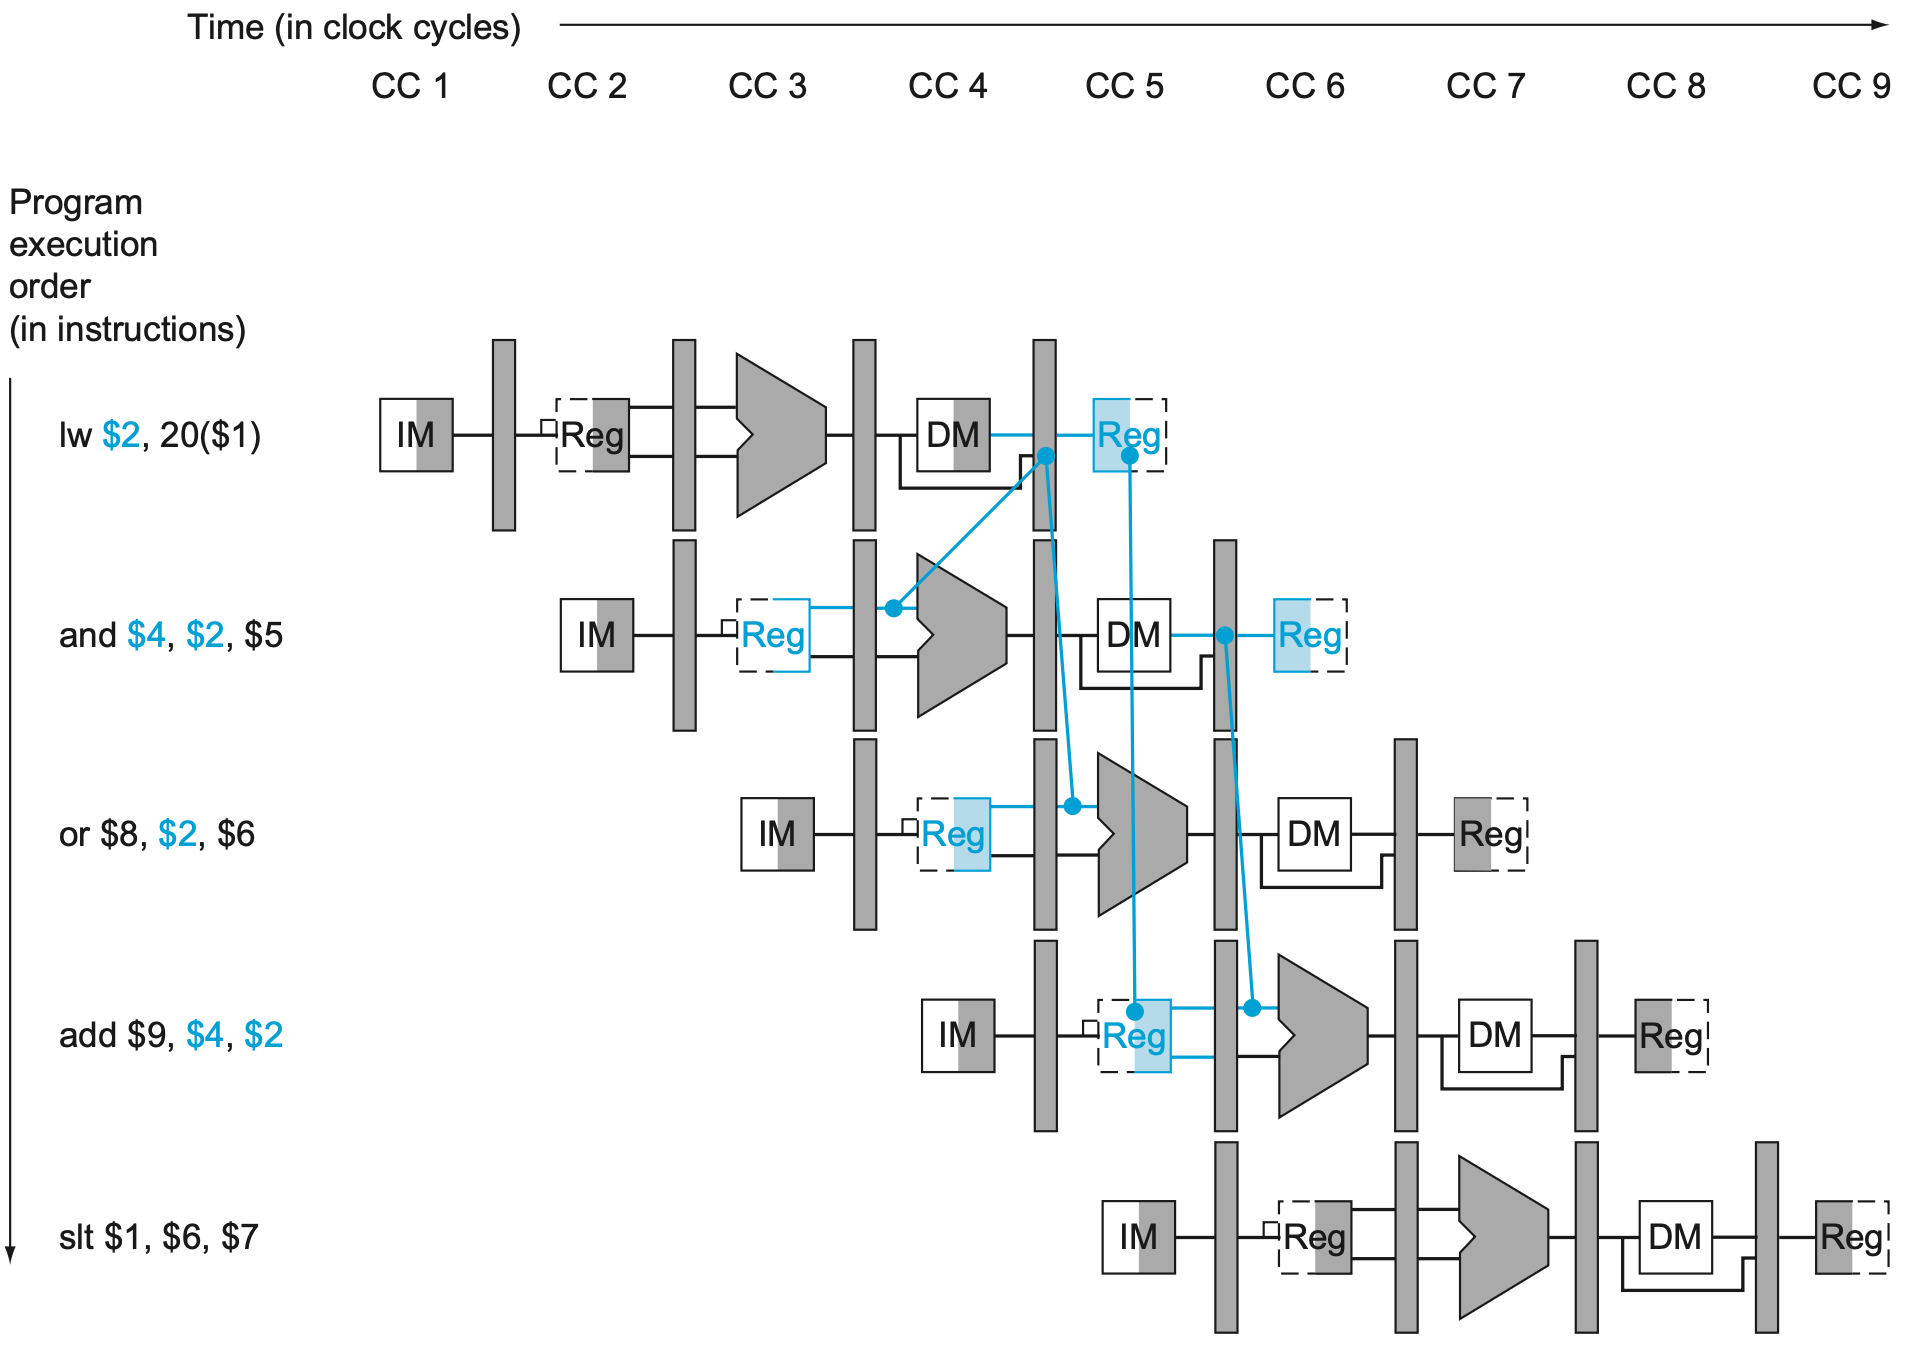
\includegraphics[width=0.8\textwidth]{Figure/pipeline_load_use.png}
\end{center}

To solve this problem, there are two main methods:

1. Insert NOP / Stall

One method is to insert NOPs or stall by waiting for the preceding instruction to complete. This can resolve the hazard, but it reduces the overall CPI (Cycles Per Instruction), which is not desirable.

2. Forwarding

The second method is comparatively better than the first. We can resolve data hazards by forwarding results as soon as they are available to where they are needed.

However, sometimes a combination of both methods is required. As shown below, after the \verb|lw| instruction, we need to use both stalling and data forwarding to ensure that the data is transferred correctly.

\begin{center}
  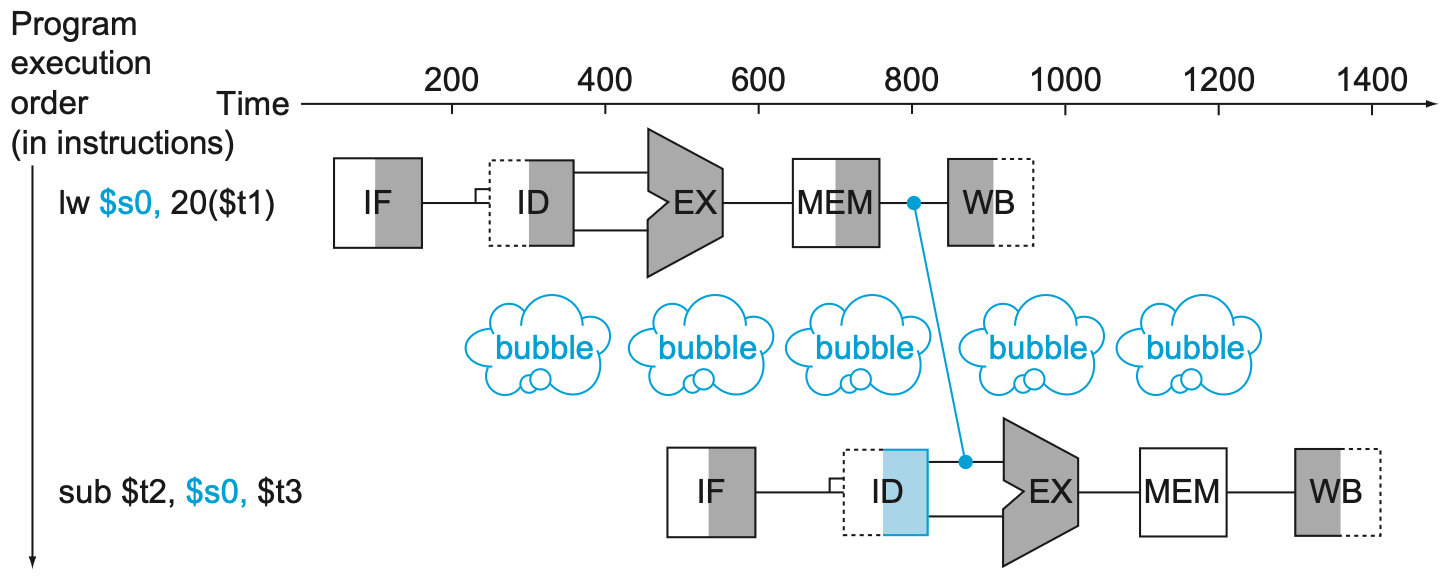
\includegraphics[width=0.8\textwidth]{Figure/pipeline_stall_forw.png}
\end{center}

Then, we can modify the datapath by adding forwarding hardware to handle data hazards more efficiently.

\begin{center}
  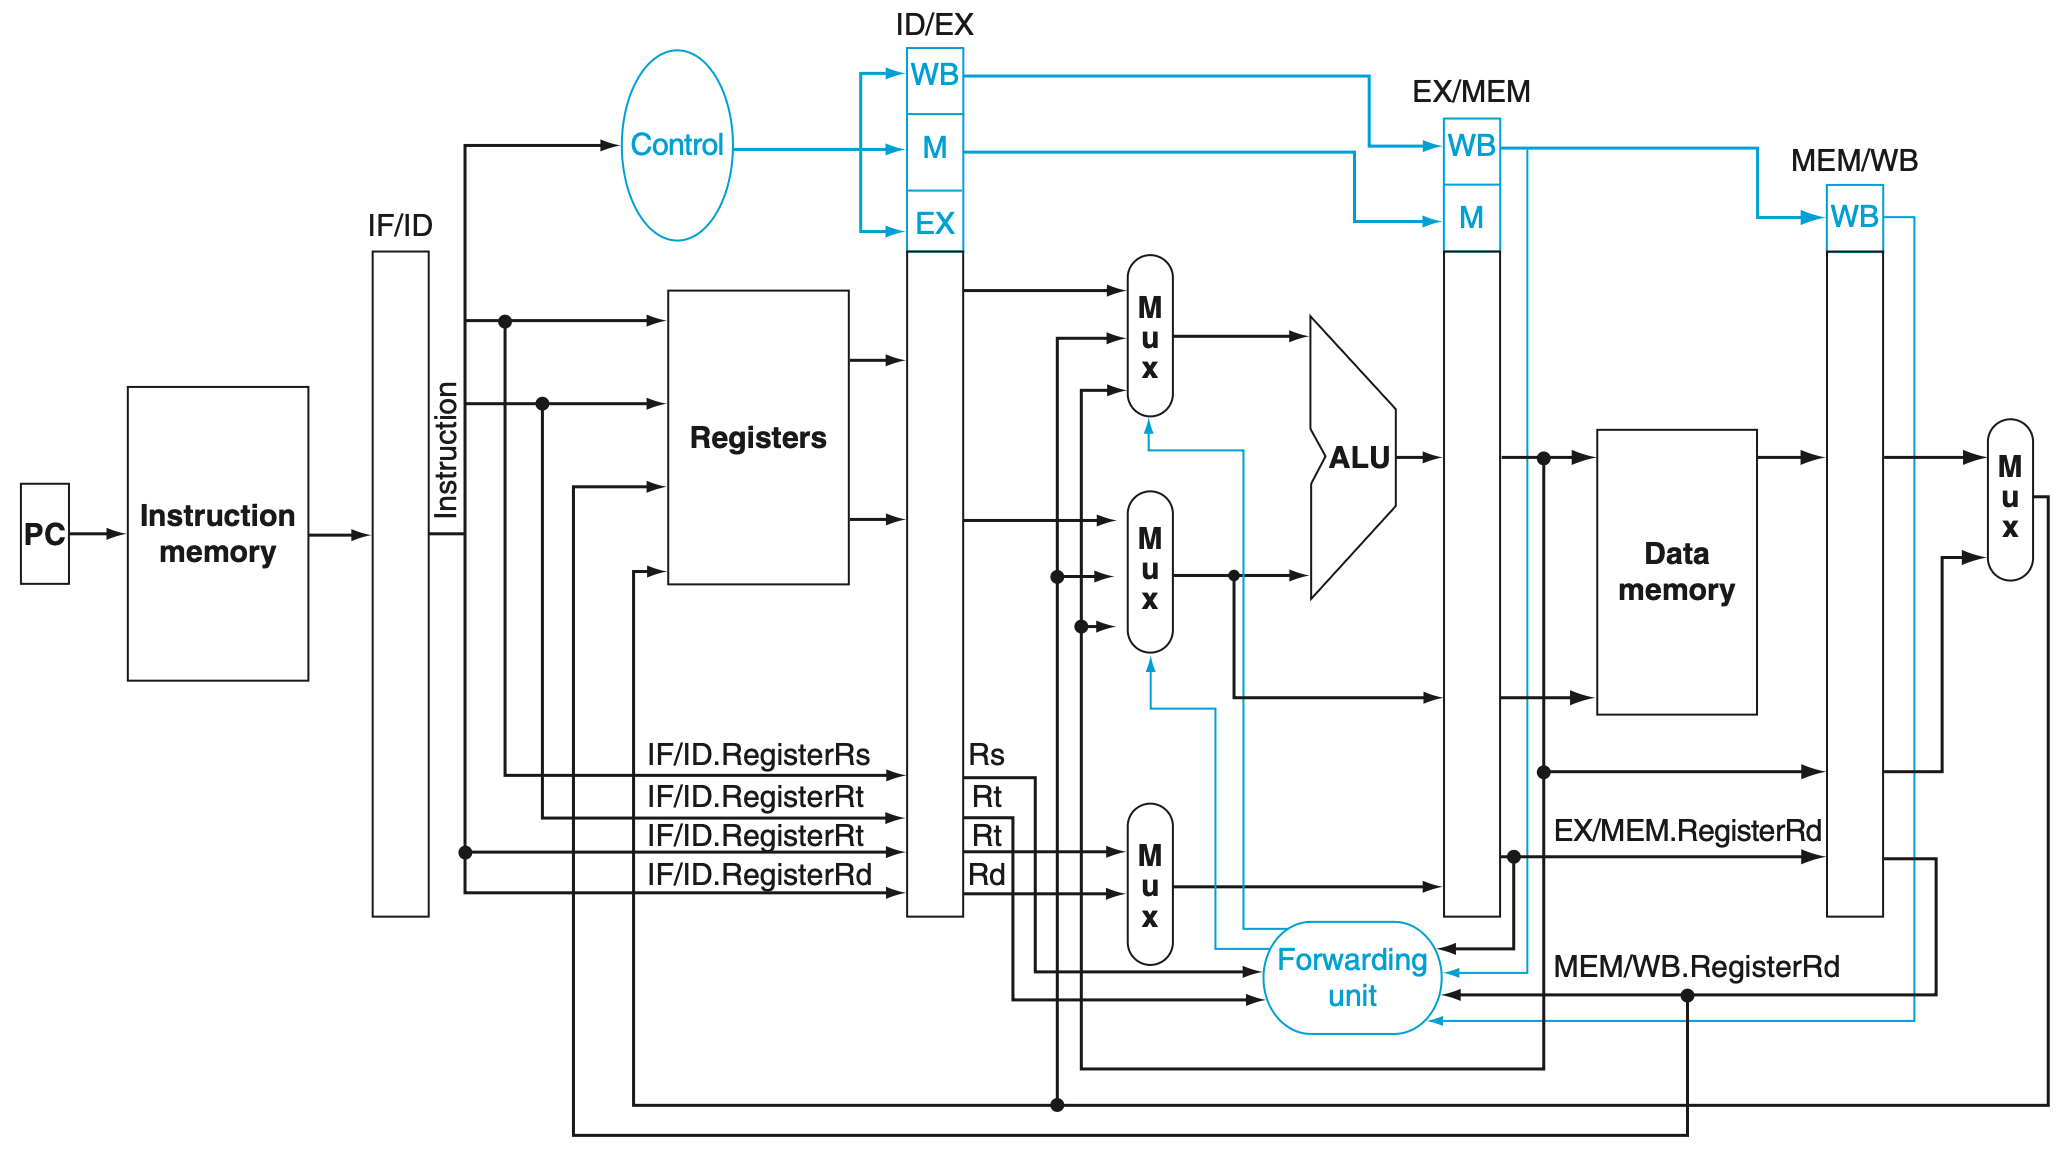
\includegraphics[width=\textwidth]{Figure/pipeline_datapath.png}
\end{center}

As mentioned before, the combination of stalling and forwarding is required for some instructions. Here is another demonstration:

\begin{center}
  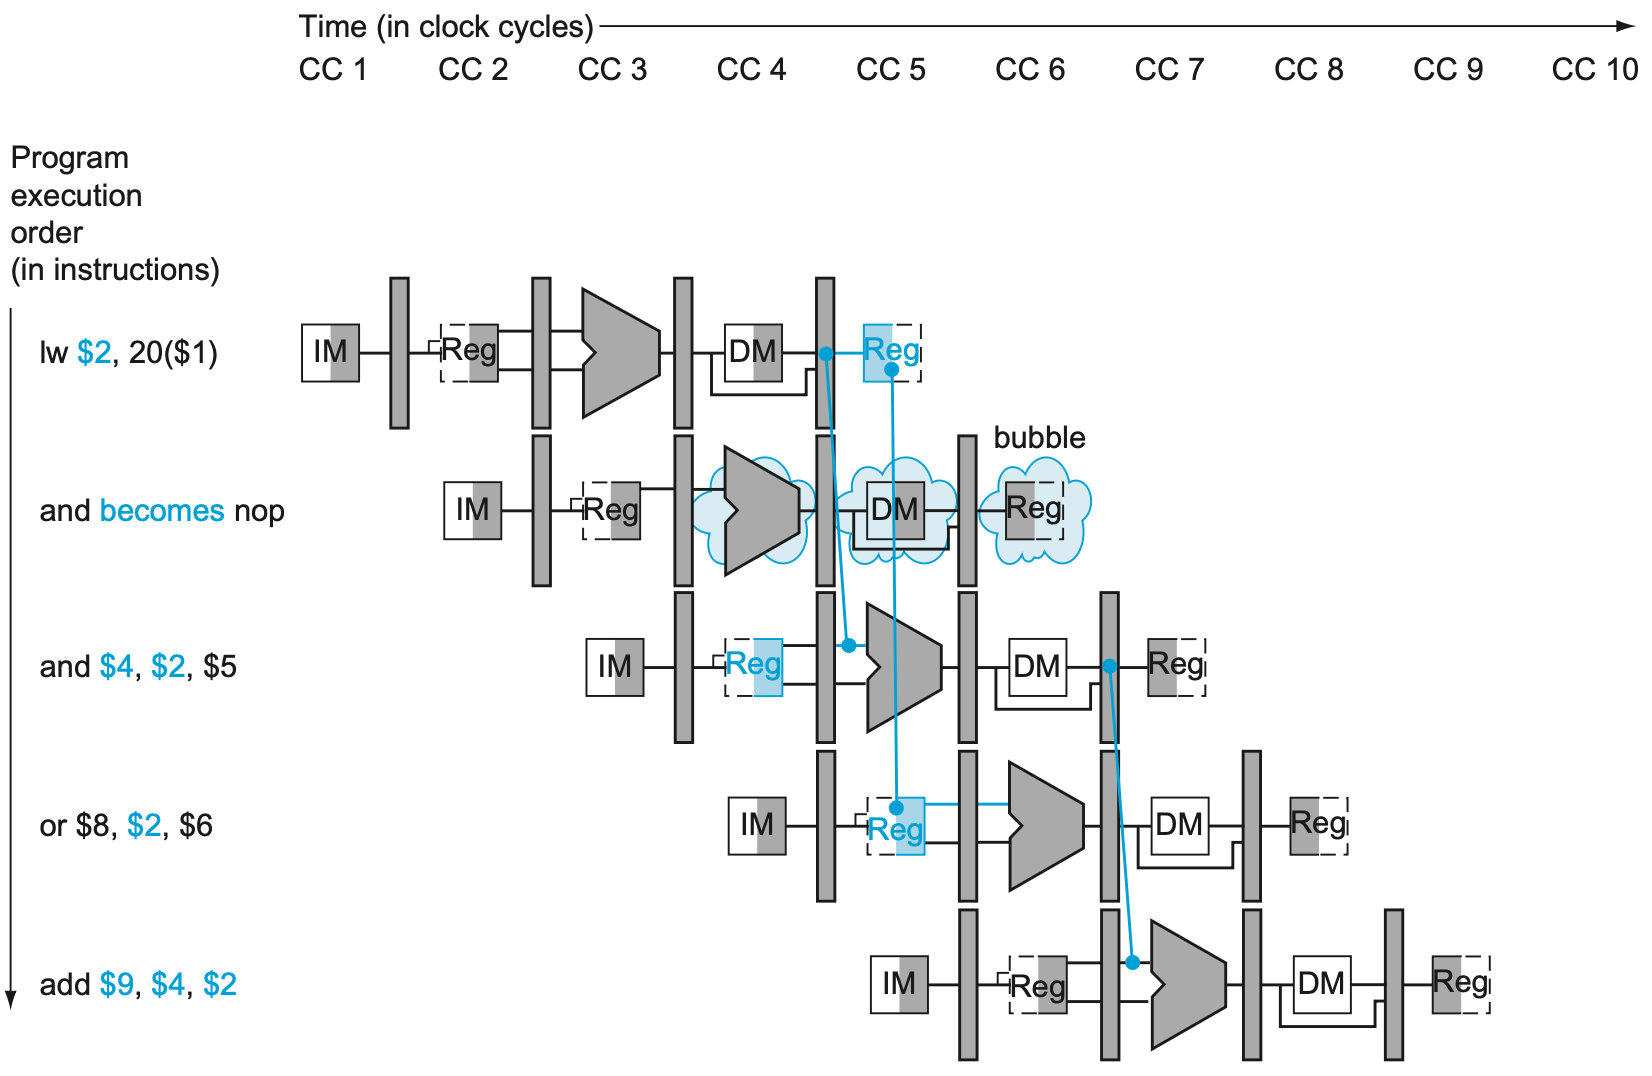
\includegraphics[width=\textwidth]{Figure/pipeline_stall_forw_2.png}
\end{center}

\section{Control Hazards}
The next type is the control hazard. Control hazards occur when the flow of instruction addresses is not sequential, arising from the need to make a decision based on the results of one instruction while others are still executing. They happen due to changes in the flow of instructions, such as:

1. Unconditional branches: \verb|jal|, \verb|jalr|

2. Conditional branches: \verb|beq|, \verb|bne|

3. Exceptions

\subsection{Pipeline Stalls}
Control hazards can be mitigated by stalling, moving the decision point as early as possible in the pipeline, delaying the decision, or using prediction techniques.

However, control hazards occur less frequently than data hazards, and there is nothing as effective against control hazards as forwarding is against data hazards.

First, we can take a look at how control hazards occur.

In jump instructions, the instruction is not decoded until the ID stage. This means that the pipeline might execute sequential instructions before determining whether the jump is taken, causing incorrect instructions to be processed due to the pipeline's nature. This results in a control hazard, and it's undesirable because the pipeline has already committed to the wrong instructions. We can fix this issue by using a single stall. 

Fortunately, jumps are relatively infrequent, reducing their impact on performance.

For branch instructions, control hazards occur due to the need to resolve the condition (e.g., whether the branch is taken or not) before proceeding with the correct instructions. This delay in knowing the outcome of the branch results in pipeline hazards, often requiring mechanisms like branch prediction to mitigate the impact.

To solve this problem, we can again use stalls. This would easily fix the issue. However, as with data hazards, it still affects the overall CPI.

\begin{remark}
  There are two types of stalls. A \textbf{NOP} instruction is inserted between two instructions in the pipeline. It prevents the instructions earlier in the pipeline from progressing down the pipeline for a cycle. A \textbf{flush} occurs when an instruction in the pipeline is replaced with a NOP instruction.
\end{remark}

\subsection{Delayed Branching}
Another method to solve this problem is by moving the branch decision hardware as early in the pipeline as possible, i.e., during the decode cycle. This will help reduce the delay of branch instructions.

To reduce the stalls, we can move the branch decision hardware back to the EX stage. This would reduce the number of stall cycles to two. Additionally, we can add hardware to compute the branch target address and evaluate the branch decision during the ID stage.

If the branch hardware is moved to the ID stage, we can eliminate all branch stalls with delayed branches. Delayed branches are defined as always executing the next sequential instruction after the branch instruction — the branch takes effect after that next instruction.

- The compiler moves an instruction that is not affected by the branch (a safe instruction) immediately after the branch, thereby hiding the branch delay.

- With deeper pipelines, the branch delay grows, requiring more than one delay slot.


- Delayed branches have lost popularity compared to more expensive but more flexible (dynamic) hardware branch prediction.

- The growth in available transistors has made hardware branch prediction relatively cheaper.

For the compiler or software, we can schedule the branch delay slots as shown below. 

Here, (a) is the best choice, as it fills the delay slot with the instruction, which reduces the IC (Instructions Count). In (b) and (c), the subtraction instruction may need to be duplicated, which increases the IC. However, they must be able to execute the subtraction when the branch fails.

\begin{center}
  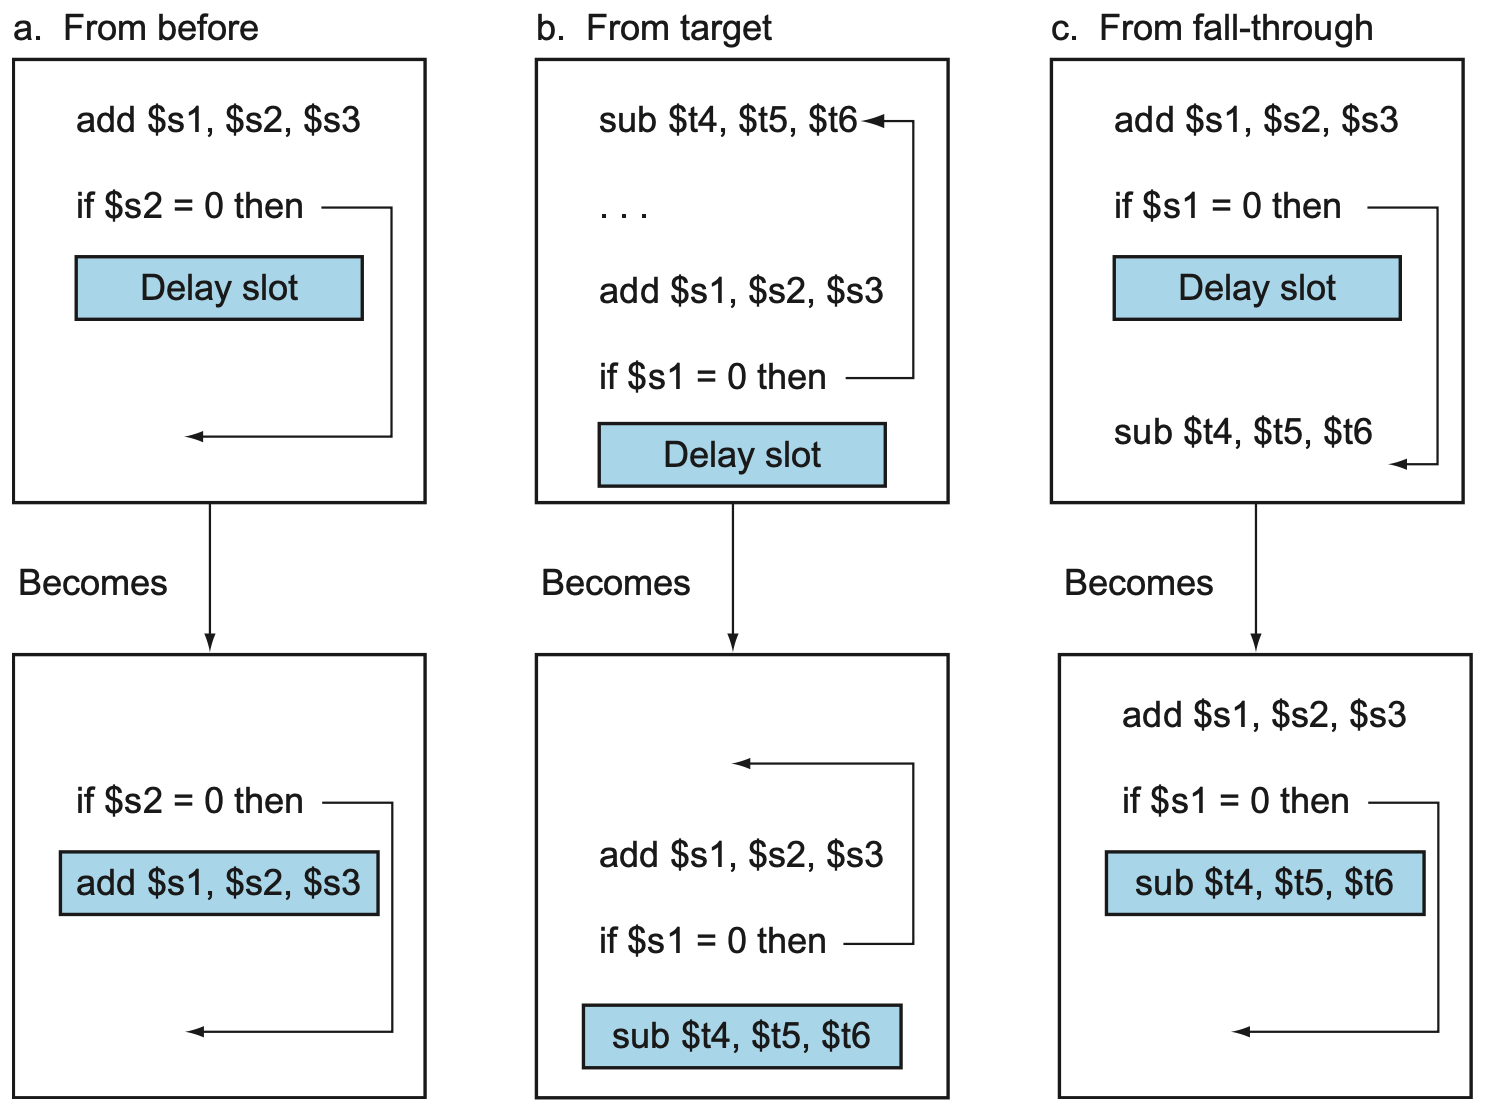
\includegraphics[width=0.7\textwidth]{Figure/branch_delay_schedule.png}
\end{center}

\subsection{Branch Prediction}
We can also use branch prediction to resolve the branch delay by assuming a given outcome and proceeding without waiting to see the actual branch outcome.

\subsubsection*{Static Branch Prediction}
One prediction we can make is "branch not taken". In this case, we always predict that branches will not be taken and continue fetching from the sequential instruction stream. Only when the branch is taken does the pipeline stall. If it is taken, we flush the instructions after the branch and restart the pipeline at the branch destination.

"Predict not taken" works well for "top of the loop" branching structures, but such loops have jumps at the bottom to return to the top, incurring the jump stall overhead. Additionally, prediction "not taken" does not work well for "bottom of the loop" branching structures.

Another prediction we could make is "branch taken." This always incurs one stall cycle. As the branch penalty increases, a simple static prediction scheme will hurt performance. With more hardware, it is possible to predict branch behavior dynamically during program execution.

\subsubsection*{Dynamic Branch Prediction}
We can also use dynamic branch prediction, where we predict branches at run-time using run-time information. This uses historical information to make more accurate predictions.

A branch prediction buffer (also known as a Branch History Table (BHT)) in the IF stage is addressed by the lower bits of the PC. It contains a bit (or bits) passed to the ID stage through the IF/ID pipeline register, indicating whether the branch was taken the last time it was executed.

The prediction bit may be incorrect (it could be a wrong prediction for this branch iteration or from a different branch with the same low-order PC bits), but this does not affect correctness—only performance.

The branch decision occurs in the ID stage after determining that the fetched instruction is a branch and checking the prediction bit(s).

If the prediction is wrong, we flush the incorrect instruction(s) in the pipeline, restart the pipeline with the correct instruction, and invert the prediction bit(s).

If the prediction is correct, stalls can be avoided no matter which direction they go.

We also have two types of predictor. 

A 1-bit predictor will be incorrect twice when not taken:
\begin{itemize}
  \item Assume \texttt{predict bit} = 0 to start (indicating branch not taken) and loop control is at the bottom of the loop code.
  \item The first time through the loop, the predictor mispredicts the branch since the branch is taken back to the top of the loop. The prediction bit is inverted (\texttt{predict bit} = 1).
  \item As long as the branch is taken (looping), the prediction is correct.
  \item Exiting the loop, the predictor again mispredicts the branch, since this time the branch is not taken (falling out of the loop). The prediction bit is inverted (\texttt{predict bit} = 0).
  \item For 10 times through the loop, we have an 80\% prediction accuracy for a branch that is taken 90\% of the time.
\end{itemize}

A 2-bit scheme can give 90\% accuracy since a prediction must be wrong twice before the prediction bit is changed.
\begin{center}
  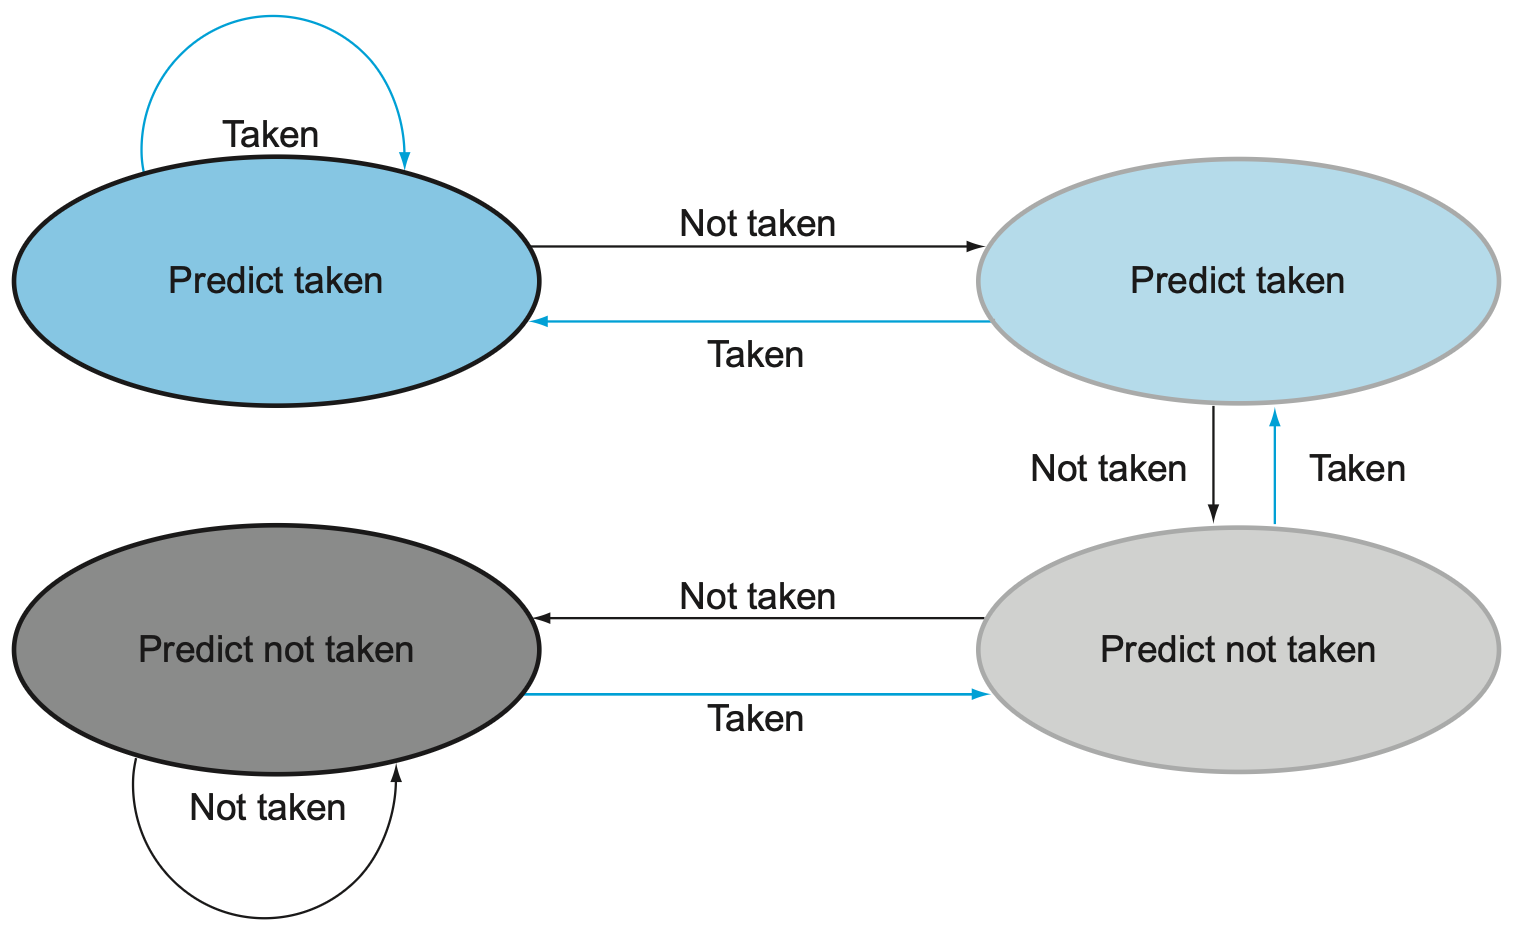
\includegraphics[width=0.5\textwidth]{Figure/branch_prediction.png}
\end{center}

\section{Exceptions}
Exceptions (also known as interrupts) are just another form of control hazard. Exceptions arise from:
\begin{itemize}
  \item R-type arithmetic overflow
  \item Trying to execute an undefined instruction
  \item An I/O device request
  \item An OS service request (e.g., a page fault, TLB exception)
  \item A hardware malfunction
\end{itemize}

The pipeline has to stop executing the offending instruction in midstream, let all prior instructions complete, flush all following instructions, set a register to show the cause of the exception, save the address of the offending instruction, and then jump to a prearranged address (the address of the exception handler code). The software (OS) looks at the cause of the exception and deals with it.

There are two types of exceptions. The first one is Interrupts, which are asynchronous to program execution. These are caused by external events and may be handled between instructions, allowing the instructions currently active in the pipeline to complete before passing control to the OS interrupt handler. We simply suspend and resume the user program.

The second type is Traps, which are synchronous to program execution. These are caused by internal events. The condition must be remedied by the trap handler for that instruction, so the offending instruction must stop midstream in the pipeline and pass control to the OS trap handler. The offending instruction may be retired, and the program may continue, or it may be aborted.

To put it simply, it's just a bug occurring in the code, and the compiler aborts. Traps are exceptions like division by zero, accessing invalid memory, etc., which are called synchronous. Interrupts are external events, like network devices needing attention, or pressing keyboard while compiling.

Notice that multiple exceptions can occur simultaneously in a single clock cycle.
